% Options for packages loaded elsewhere
\PassOptionsToPackage{unicode}{hyperref}
\PassOptionsToPackage{hyphens}{url}
\PassOptionsToPackage{dvipsnames,svgnames,x11names}{xcolor}
%
\documentclass[
  letterpaper,
  DIV=11,
  numbers=noendperiod]{scrartcl}

\usepackage{amsmath,amssymb}
\usepackage{iftex}
\ifPDFTeX
  \usepackage[T1]{fontenc}
  \usepackage[utf8]{inputenc}
  \usepackage{textcomp} % provide euro and other symbols
\else % if luatex or xetex
  \usepackage{unicode-math}
  \defaultfontfeatures{Scale=MatchLowercase}
  \defaultfontfeatures[\rmfamily]{Ligatures=TeX,Scale=1}
\fi
\usepackage{lmodern}
\ifPDFTeX\else  
    % xetex/luatex font selection
\fi
% Use upquote if available, for straight quotes in verbatim environments
\IfFileExists{upquote.sty}{\usepackage{upquote}}{}
\IfFileExists{microtype.sty}{% use microtype if available
  \usepackage[]{microtype}
  \UseMicrotypeSet[protrusion]{basicmath} % disable protrusion for tt fonts
}{}
\makeatletter
\@ifundefined{KOMAClassName}{% if non-KOMA class
  \IfFileExists{parskip.sty}{%
    \usepackage{parskip}
  }{% else
    \setlength{\parindent}{0pt}
    \setlength{\parskip}{6pt plus 2pt minus 1pt}}
}{% if KOMA class
  \KOMAoptions{parskip=half}}
\makeatother
\usepackage{xcolor}
\setlength{\emergencystretch}{3em} % prevent overfull lines
\setcounter{secnumdepth}{-\maxdimen} % remove section numbering
% Make \paragraph and \subparagraph free-standing
\makeatletter
\ifx\paragraph\undefined\else
  \let\oldparagraph\paragraph
  \renewcommand{\paragraph}{
    \@ifstar
      \xxxParagraphStar
      \xxxParagraphNoStar
  }
  \newcommand{\xxxParagraphStar}[1]{\oldparagraph*{#1}\mbox{}}
  \newcommand{\xxxParagraphNoStar}[1]{\oldparagraph{#1}\mbox{}}
\fi
\ifx\subparagraph\undefined\else
  \let\oldsubparagraph\subparagraph
  \renewcommand{\subparagraph}{
    \@ifstar
      \xxxSubParagraphStar
      \xxxSubParagraphNoStar
  }
  \newcommand{\xxxSubParagraphStar}[1]{\oldsubparagraph*{#1}\mbox{}}
  \newcommand{\xxxSubParagraphNoStar}[1]{\oldsubparagraph{#1}\mbox{}}
\fi
\makeatother


\providecommand{\tightlist}{%
  \setlength{\itemsep}{0pt}\setlength{\parskip}{0pt}}\usepackage{longtable,booktabs,array}
\usepackage{calc} % for calculating minipage widths
% Correct order of tables after \paragraph or \subparagraph
\usepackage{etoolbox}
\makeatletter
\patchcmd\longtable{\par}{\if@noskipsec\mbox{}\fi\par}{}{}
\makeatother
% Allow footnotes in longtable head/foot
\IfFileExists{footnotehyper.sty}{\usepackage{footnotehyper}}{\usepackage{footnote}}
\makesavenoteenv{longtable}
\usepackage{graphicx}
\makeatletter
\def\maxwidth{\ifdim\Gin@nat@width>\linewidth\linewidth\else\Gin@nat@width\fi}
\def\maxheight{\ifdim\Gin@nat@height>\textheight\textheight\else\Gin@nat@height\fi}
\makeatother
% Scale images if necessary, so that they will not overflow the page
% margins by default, and it is still possible to overwrite the defaults
% using explicit options in \includegraphics[width, height, ...]{}
\setkeys{Gin}{width=\maxwidth,height=\maxheight,keepaspectratio}
% Set default figure placement to htbp
\makeatletter
\def\fps@figure{htbp}
\makeatother
% definitions for citeproc citations
\NewDocumentCommand\citeproctext{}{}
\NewDocumentCommand\citeproc{mm}{%
  \begingroup\def\citeproctext{#2}\cite{#1}\endgroup}
\makeatletter
 % allow citations to break across lines
 \let\@cite@ofmt\@firstofone
 % avoid brackets around text for \cite:
 \def\@biblabel#1{}
 \def\@cite#1#2{{#1\if@tempswa , #2\fi}}
\makeatother
\newlength{\cslhangindent}
\setlength{\cslhangindent}{1.5em}
\newlength{\csllabelwidth}
\setlength{\csllabelwidth}{3em}
\newenvironment{CSLReferences}[2] % #1 hanging-indent, #2 entry-spacing
 {\begin{list}{}{%
  \setlength{\itemindent}{0pt}
  \setlength{\leftmargin}{0pt}
  \setlength{\parsep}{0pt}
  % turn on hanging indent if param 1 is 1
  \ifodd #1
   \setlength{\leftmargin}{\cslhangindent}
   \setlength{\itemindent}{-1\cslhangindent}
  \fi
  % set entry spacing
  \setlength{\itemsep}{#2\baselineskip}}}
 {\end{list}}
\usepackage{calc}
\newcommand{\CSLBlock}[1]{\hfill\break\parbox[t]{\linewidth}{\strut\ignorespaces#1\strut}}
\newcommand{\CSLLeftMargin}[1]{\parbox[t]{\csllabelwidth}{\strut#1\strut}}
\newcommand{\CSLRightInline}[1]{\parbox[t]{\linewidth - \csllabelwidth}{\strut#1\strut}}
\newcommand{\CSLIndent}[1]{\hspace{\cslhangindent}#1}

\KOMAoption{captions}{tableheading}
\makeatletter
\@ifpackageloaded{tcolorbox}{}{\usepackage[skins,breakable]{tcolorbox}}
\@ifpackageloaded{fontawesome5}{}{\usepackage{fontawesome5}}
\definecolor{quarto-callout-color}{HTML}{909090}
\definecolor{quarto-callout-note-color}{HTML}{0758E5}
\definecolor{quarto-callout-important-color}{HTML}{CC1914}
\definecolor{quarto-callout-warning-color}{HTML}{EB9113}
\definecolor{quarto-callout-tip-color}{HTML}{00A047}
\definecolor{quarto-callout-caution-color}{HTML}{FC5300}
\definecolor{quarto-callout-color-frame}{HTML}{acacac}
\definecolor{quarto-callout-note-color-frame}{HTML}{4582ec}
\definecolor{quarto-callout-important-color-frame}{HTML}{d9534f}
\definecolor{quarto-callout-warning-color-frame}{HTML}{f0ad4e}
\definecolor{quarto-callout-tip-color-frame}{HTML}{02b875}
\definecolor{quarto-callout-caution-color-frame}{HTML}{fd7e14}
\makeatother
\makeatletter
\@ifpackageloaded{caption}{}{\usepackage{caption}}
\AtBeginDocument{%
\ifdefined\contentsname
  \renewcommand*\contentsname{Table of contents}
\else
  \newcommand\contentsname{Table of contents}
\fi
\ifdefined\listfigurename
  \renewcommand*\listfigurename{List of Figures}
\else
  \newcommand\listfigurename{List of Figures}
\fi
\ifdefined\listtablename
  \renewcommand*\listtablename{List of Tables}
\else
  \newcommand\listtablename{List of Tables}
\fi
\ifdefined\figurename
  \renewcommand*\figurename{Figure}
\else
  \newcommand\figurename{Figure}
\fi
\ifdefined\tablename
  \renewcommand*\tablename{Table}
\else
  \newcommand\tablename{Table}
\fi
}
\@ifpackageloaded{float}{}{\usepackage{float}}
\floatstyle{ruled}
\@ifundefined{c@chapter}{\newfloat{codelisting}{h}{lop}}{\newfloat{codelisting}{h}{lop}[chapter]}
\floatname{codelisting}{Listing}
\newcommand*\listoflistings{\listof{codelisting}{List of Listings}}
\makeatother
\makeatletter
\makeatother
\makeatletter
\@ifpackageloaded{caption}{}{\usepackage{caption}}
\@ifpackageloaded{subcaption}{}{\usepackage{subcaption}}
\makeatother

\ifLuaTeX
  \usepackage{selnolig}  % disable illegal ligatures
\fi
\usepackage{bookmark}

\IfFileExists{xurl.sty}{\usepackage{xurl}}{} % add URL line breaks if available
\urlstyle{same} % disable monospaced font for URLs
\hypersetup{
  pdftitle={Survey Quality Predictor},
  pdfauthor={Lukas Birkenmaier; Lydia Repke; Cem Eryar},
  colorlinks=true,
  linkcolor={blue},
  filecolor={Maroon},
  citecolor={Blue},
  urlcolor={Blue},
  pdfcreator={LaTeX via pandoc}}


\title{Survey Quality Predictor}
\usepackage{etoolbox}
\makeatletter
\providecommand{\subtitle}[1]{% add subtitle to \maketitle
  \apptocmd{\@title}{\par {\large #1 \par}}{}{}
}
\makeatother
\subtitle{A survey quality prediction system for continuous questions
used in survey research}
\author{Lukas Birkenmaier \and Lydia Repke \and Cem Eryar}
\date{Invalid Date}

\begin{document}
\maketitle


\section{Introduction}\label{introduction}

The Survey Quality Predictor (SQP) 3.0 is an open-access system for
predicting the reliability, validity, and quality of survey questions
for continuous latent variables based on their formal and linguistic
characteristics (such as the properties of the answer scale and the
administration mode). SQP is grounded in decades of methodological
research and enables survey designers and researchers to evaluate and
enhance the quality of their measurement instruments. By systematically
linking the characteristics of survey items to their measurement
quality, SQP provides a practical framework for improving data quality
in survey-based research (Felderer et al., 2024).

Relying on SQP's prediction power and its day-by-day extending database,
researchers can effectively utilize its features in at least three
different ways (Felderer et al., 2024):

\begin{itemize}
\item
  During the questionnaire development process, researchers can consult
  the database, predict the qualities of different item versions, and
  make informed comparisons.
\item
  SQP enables researchers to compare different language versions of the
  same item by analyzing the coded characteristics. This analysis helps
  identify potential methodological differences between the source items
  and their translations, thus supporting quality control of
  translations in cross-cultural surveys.
\item
  SQP's quality predictions can be used in substantial analyses to
  correct for measurement errors of items capturing subjective concepts
  (Andrews, 1984; Saris et al., 2022; Saris \& Revilla, 2016).
\end{itemize}

In this tutorial, we will explain the conceptual framework of SQP,
demonstrate its function through an example, and conclude with a
discussion on its benefits, limitations, and potential for future
development. Overall, this tutorial aims to ensure that survey designers
and researchers can harness SQP to create better surveys, mitigate
potential biases, and enhance the overall quality of their research.

\section{SQP}\label{sqp}

The Survey Quality Predictor (SQP) is a software tool developed to
predict the measurement quality of survey items for continuous latent
variables. It operates by analyzing survey items' formal and linguistic
characteristics (GESIS -- Leibniz Institute for the Social Sciences,
2024). SQP's development is rooted in decades of methodological
research, beginning in the 1980s when Willem Saris and his colleagues
conducted a series of multitrait-multimethod (MTMM) experiments. These
experiments aimed to quantify the reliability and validity of survey
items and disentangle random and systematic errors, ultimately improving
the quality of survey instruments (Saris \& Gallhofer, 2014). The
insights from these early experiments laid the foundation for SQP's
predictive capabilities.

The first version of SQP was released in 2001 (\textbf{saris2001?}).
This version operationalized the findings from MTMM research into a
practical tool that allowed users to code survey items and predict their
reliability and validity. While groundbreaking, SQP 1.0 had limitations,
such as a relatively small database on which the prediction was based
and a lack of advanced features (GESIS -- Leibniz Institute for the
Social Sciences, 2024). A decade later, SQP 2.0 introduced significant
advancements, including an expanded database and a new prediction
algorithm. In 2015, SQP received a usability makeover, improving the
user experience as version 2.1 (Saris et al., 2022). The release of SQP
3.0 in 2022 marked a major milestone in survey research methodology.
This version included thousands of survey items coded in 28 languages
for 33 countries, making it particularly valuable for cross-cultural and
multilingual studies like the European Social Survey (ESS). Its updated
prediction algorithm accounted for interactions between item
characteristics, offering more accurate reliability and validity
estimates. SQP 3.0 also introduced new features that improved and
enhanced the user experience (GESIS -- Leibniz Institute for the Social
Sciences, 2024).

SQP has evolved into a comprehensive tool that supports survey
researchers in designing high-quality questionnaires, ensuring
cross-cultural comparability, and improving the quality of survey
questions. Its integration of predictive modeling, and user-friendly
features positions SQP as an indispensable resource in modern survey
research.

\subsection{The Impact of Survey Question Design and the Role of
SQP}\label{the-impact-of-survey-question-design-and-the-role-of-sqp}

The decisions made in designing survey questions significantly impact
respondents' answer behavior, as variations in question formulation,
response scales, and contextual features influence how individuals
interpret and respond to survey items. For instance, Saris et al. (2022)
illustrate this with an example of measuring trust in the economy. They
compare the effects of three different response scale designs on the
question:

\paragraph{(Q1) On the whole, how satisfied are you with the present
state of the economy in
Britain?}\label{q1-on-the-whole-how-satisfied-are-you-with-the-present-state-of-the-economy-in-britain}

\textbf{4-point bipolar scale:}

\begin{enumerate}
\def\labelenumi{\arabic{enumi}.}
\tightlist
\item
  Very satisfied\\
\item
  Satisfied\\
\item
  Dissatisfied\\
\item
  Very dissatisfied
\end{enumerate}

\textbf{4-point unipolar scale:}

\begin{enumerate}
\def\labelenumi{\arabic{enumi}.}
\tightlist
\item
  Not at all satisfied\\
\item
  Satisfied\\
\item
  Rather satisfied\\
\item
  Very satisfied
\end{enumerate}

\textbf{Numeric Scale (0--10):}

The results revealed significant differences in response distributions
and correlations with related variables based on the scale used. For
instance, numeric scales tended to produce higher correlations with
other trust measures, whereas bipolar and unipolar scales generated
distinct response patterns. These variations stem from the way survey
questions influence respondents' cognitive processing.

Bipolar scales emphasize contrasts between extremes, potentially
encouraging more polarized responses, while unipolar scales direct
attention to a single dimension, which may reduce polarization but
introduce other biases. In contrast, numeric scales convey a sense of
precision and neutrality yet require respondents to map their attitudes
onto a numeric continuum. These subtle but impactful differences
highlight the critical role of thoughtful survey design, especially for
subjective constructs like trust or satisfaction (Saris et al., 2022).

Therefore, SQP is essential for ensuring high-quality survey research,
as it systematically addresses the impact of question design on
measurement outcomes. By predicting the reliability and validity of
survey questions, SQP helps researchers identify potential biases and
unintended effects introduced by variations in scales, wording, or
structure. For example, as demonstrated by differences between numeric,
bipolar, and unipolar scales, minor design changes can profoundly
influence respondents' cognitive processing and, consequently, the data
collected. This is particularly critical for subjective measures like
trust, satisfaction, or attitudes, where nuanced design decisions can
significantly affect data quality and the validity of subsequent
analyses.

\subsection{Introduction to the Coding Process in
SQP}\label{introduction-to-the-coding-process-in-sqp}

The SQP Website provides researchers with a comprehensive tool to
evaluate and enhance the quality of survey questions systematically. At
the heart of this process lies the coding of survey items, where
specific characteristics of questions are analyzed to generate
predictions about their reliability and validity. The SQP website offers
an intuitive interface that facilitates both the coding process and
access to its extensive database of survey items.

To use the tool's full functionality, researchers must
\href{https://sqp.gesis.org/signin}{register} and create an account on
the platform. Once logged in, they can interact with a searchable
database containing a vast collection of survey items from various
studies, languages, and countries, add new survey questions, and code
them to get quality predictions.

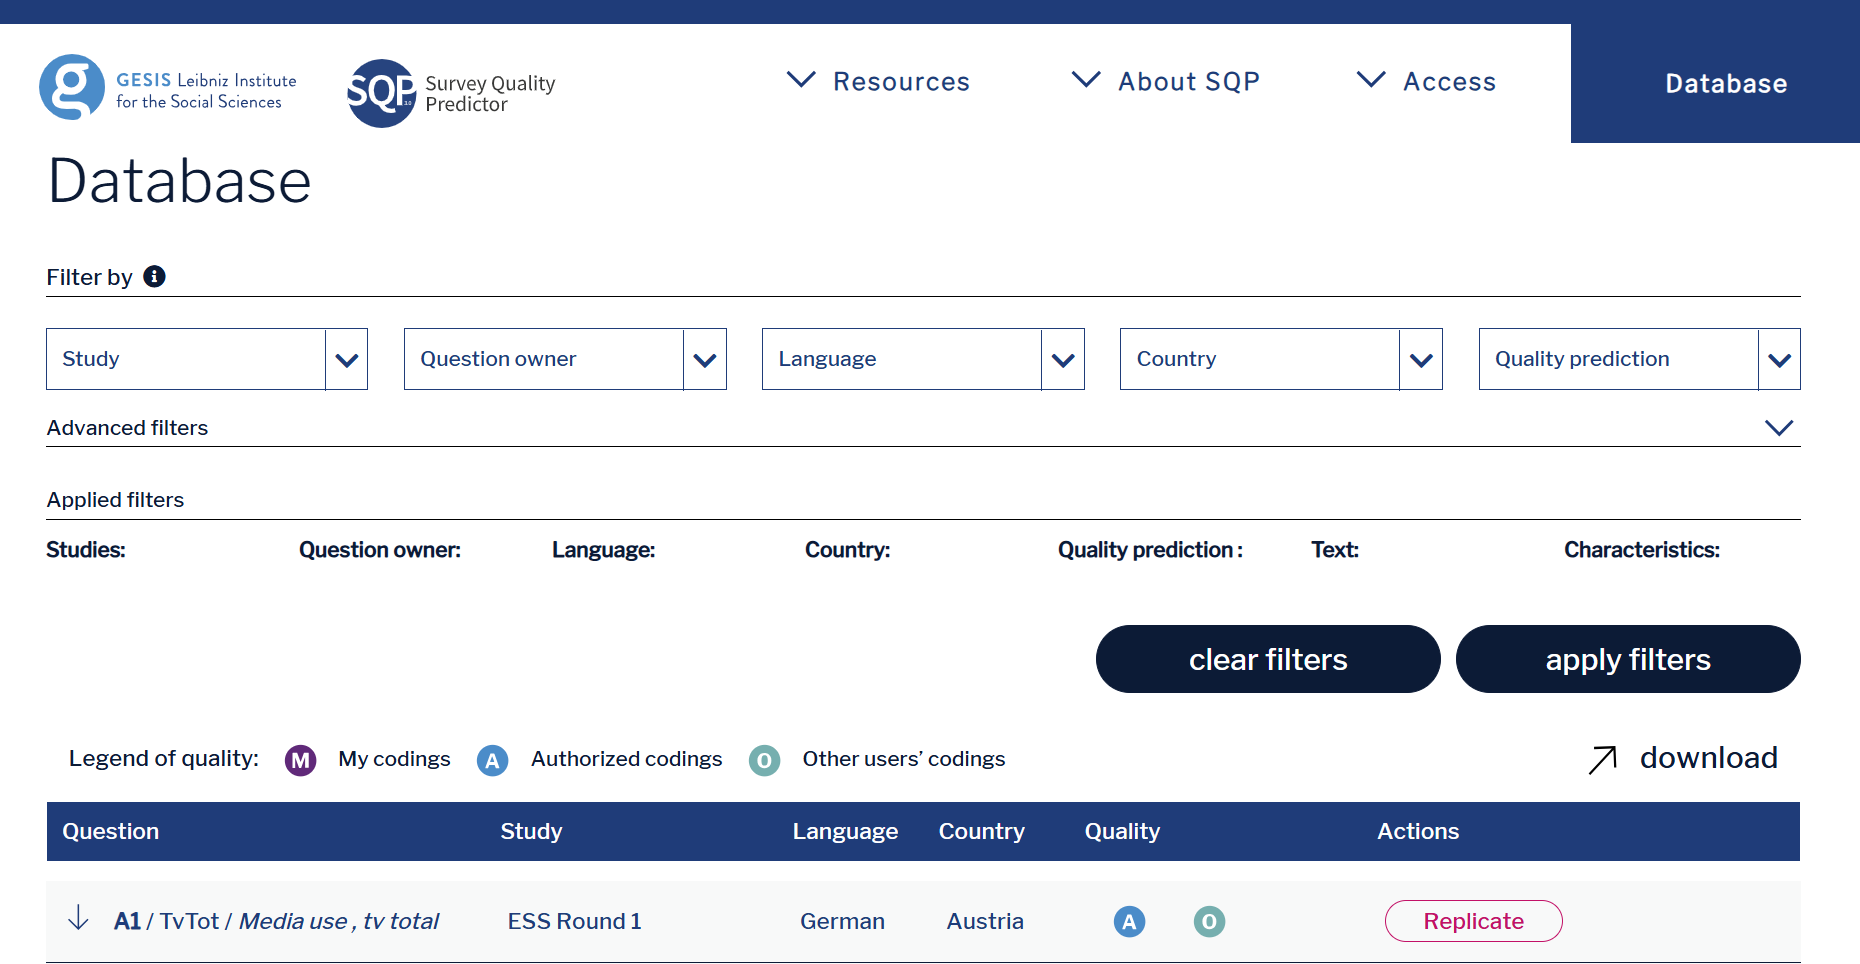
\includegraphics{img/landing_page.png}

The database allows researchers to explore existing items, apply
filters, and use advanced search options to focus on specific topics or
coding characteristics. For instance, users interested in survey items
coded for ``centrality'' or measuring concepts like ``political
efficacy'' can refine their search accordingly.

As mentioned above, the platform further enables researchers to
contribute to the database with new survey items by entering key
details, such as the question text, response options, and metadata about
the study. After adding an item, users proceed to the coding stage,
where they thoroughly analyze the survey question's characteristics.
This process involves evaluating features like the response scale,
linguistic complexity, and the formulation of the request for an answer.

\begin{tcolorbox}[enhanced jigsaw, titlerule=0mm, breakable, toptitle=1mm, leftrule=.75mm, colbacktitle=quarto-callout-note-color!10!white, colback=white, left=2mm, opacitybacktitle=0.6, rightrule=.15mm, opacityback=0, colframe=quarto-callout-note-color-frame, bottomrule=.15mm, arc=.35mm, bottomtitle=1mm, title=\textcolor{quarto-callout-note-color}{\faInfo}\hspace{0.5em}{List of Characteristics}, toprule=.15mm, coltitle=black]

\begin{longtable}[]{@{}
  >{\raggedright\arraybackslash}p{(\columnwidth - 2\tabcolsep) * \real{0.2222}}
  >{\raggedright\arraybackslash}p{(\columnwidth - 2\tabcolsep) * \real{0.7778}}@{}}
\toprule\noalign{}
\begin{minipage}[b]{\linewidth}\raggedright
\textbf{Variable Name}
\end{minipage} & \begin{minipage}[b]{\linewidth}\raggedright
\textbf{Description}
\end{minipage} \\
\midrule\noalign{}
\endhead
\bottomrule\noalign{}
\endlastfoot
\textbf{Domain} & The topic of the assertion that one wants to measure
using this survey item, determined by the research goal. \\
\textbf{Concept} & The concept one wants to measure, classified as one
of the basic concepts distinguished in SQP. \\
\textbf{Social desirability} & Relates to the domain choice; identifies
sensitive or delicate items that can bias responses. \\
\textbf{Centrality} & Measures the familiarity of respondents with the
topic, linked to the domain choice. \\
\textbf{Reference period} & Refers to the time period mentioned in the
request, e.g., present, past, or future. \\
\textbf{Formulation of the request} & The basic formulation of the
request, e.g., direct, indirect, or omitted in item batteries. \\
\textbf{WH word used in the request} & Requests starting with words like
who, what, when, where, how, etc., or their translations. \\
\textbf{Request for an answer type} & Requests may be formulated as
interrogative, imperative, or declarative. \\
\textbf{Use of gradation} & Identifies requests where responses can be
ordered, e.g., low to high or vice versa. \\
\textbf{Balance of the request} & Determines whether requests are
balanced (mentioning both poles) or unbalanced. \\
\textbf{Presence of encouragement} & Encourages responses, e.g.,
`Please, tell me\ldots{}' or `We would like to ask you\ldots{}' \\
\textbf{Emphasis on subjective opinion} & Focuses on subjective opinion,
e.g., `What do you think about\ldots?' or `According to you\ldots{}' \\
\textbf{Information regarding others' opinions} & Includes information
on others' opinions, e.g., `Some people are against nuclear energy while
others support it.' \\
\textbf{Use of stimulus or statement} & Survey items with a stimulus
(noun/words) or statements (complete sentences). \\
\textbf{Absolute or comparative judgment} & Determines whether
respondents provide absolute or comparative judgments. \\
\textbf{Response scale: basic choice} & The type of response options,
e.g., two-category, more-step procedures, open-ended, etc. \\
\textbf{Response scale characteristics} & Characteristics like number of
categories, maximum values, labels, and scale range. \\
\textbf{Don't know option} & Indicates whether a `Don't know' option is
present. \\
\textbf{Interviewer instruction} & Instructions provided to
interviewers, e.g., about showcards or visual aids. \\
\textbf{Respondent instruction} & Instructions provided to respondents,
usually in imperative or polite forms. \\
\textbf{Extra information or definition} & Additional information or
definitions provided for clarity, though not strictly necessary. \\
\textbf{Knowledge provided} & Defines whether definitions, explanations,
or both are provided. \\
\textbf{Introduction available} & Introduces the survey topic or related
questions, often at the beginning. \\
\textbf{Linguistic characteristics} & Covers linguistic features of
introduction, request, and answer scale, e.g., number of sentences,
words, or abstract nouns. \\
\textbf{Showcard used} & Indicates whether a showcard is used for
response options or additional assistance. \\
\textbf{Showcard characteristics} & Details characteristics of
showcards, e.g., scale orientation, labels, or numbers. \\
\textbf{Computer-assisted} & Indicates whether the mode of data
collection is computer-assisted. \\
\textbf{Interviewer} & Specifies whether the mode is
interviewer-administered or self-administered. \\
\textbf{Visual or oral presentation} & States whether the questionnaire
is visually presented or orally read to respondents. \\
\textbf{Position} & Indicates the position of the survey item within the
questionnaire. \\
\end{longtable}

\end{tcolorbox}

Although coding between 30 and 60 characteristics may seem daunting
initially, the platform provides clear instructions and contextual help
to guide users through the process.

Once the coding is complete, SQP generates a prediction of the item's
measurement quality, including its reliability, validity, and potential
method effects. Furthermore, the platform includes the function to
compare codings across different survey items or variations of the same
item, highlighting how design choices can influence measurement quality.
SQP also supports transparency and replicability by enabling users to
document their own survey questions and coding decisions. These features
are particularly beneficial for longitudinal or comparative research,
where consistent question design is critical.

For a detailed explanation of the coding process and additional
resources, see the full SQP guideline here:
\href{https://sqp.gesis.org/static/files/UserManualSQP-3-Version-1.pdf}{SQP
Manual}.

\subsection{Practical Application of
SQP}\label{practical-application-of-sqp}

To illustrate how measuring the same construct can vary depending on the
type of question and the answer scale used---and how these variations
can lead to different quality prediction scores---we examine a question
on economic satisfaction from Round 4 of the European Social Survey
(ESS). You can
\href{https://sqp.gesis.org/user/database?a=1&si=4&ow=&la=&co=78&q=&chv=&t=Political+satisfaction&fmcf=&fccf=&_csrf=635a1b56-6247-4b74-aae7-abfd5e3d7c0e}{click
here} to access the questions in the example below.

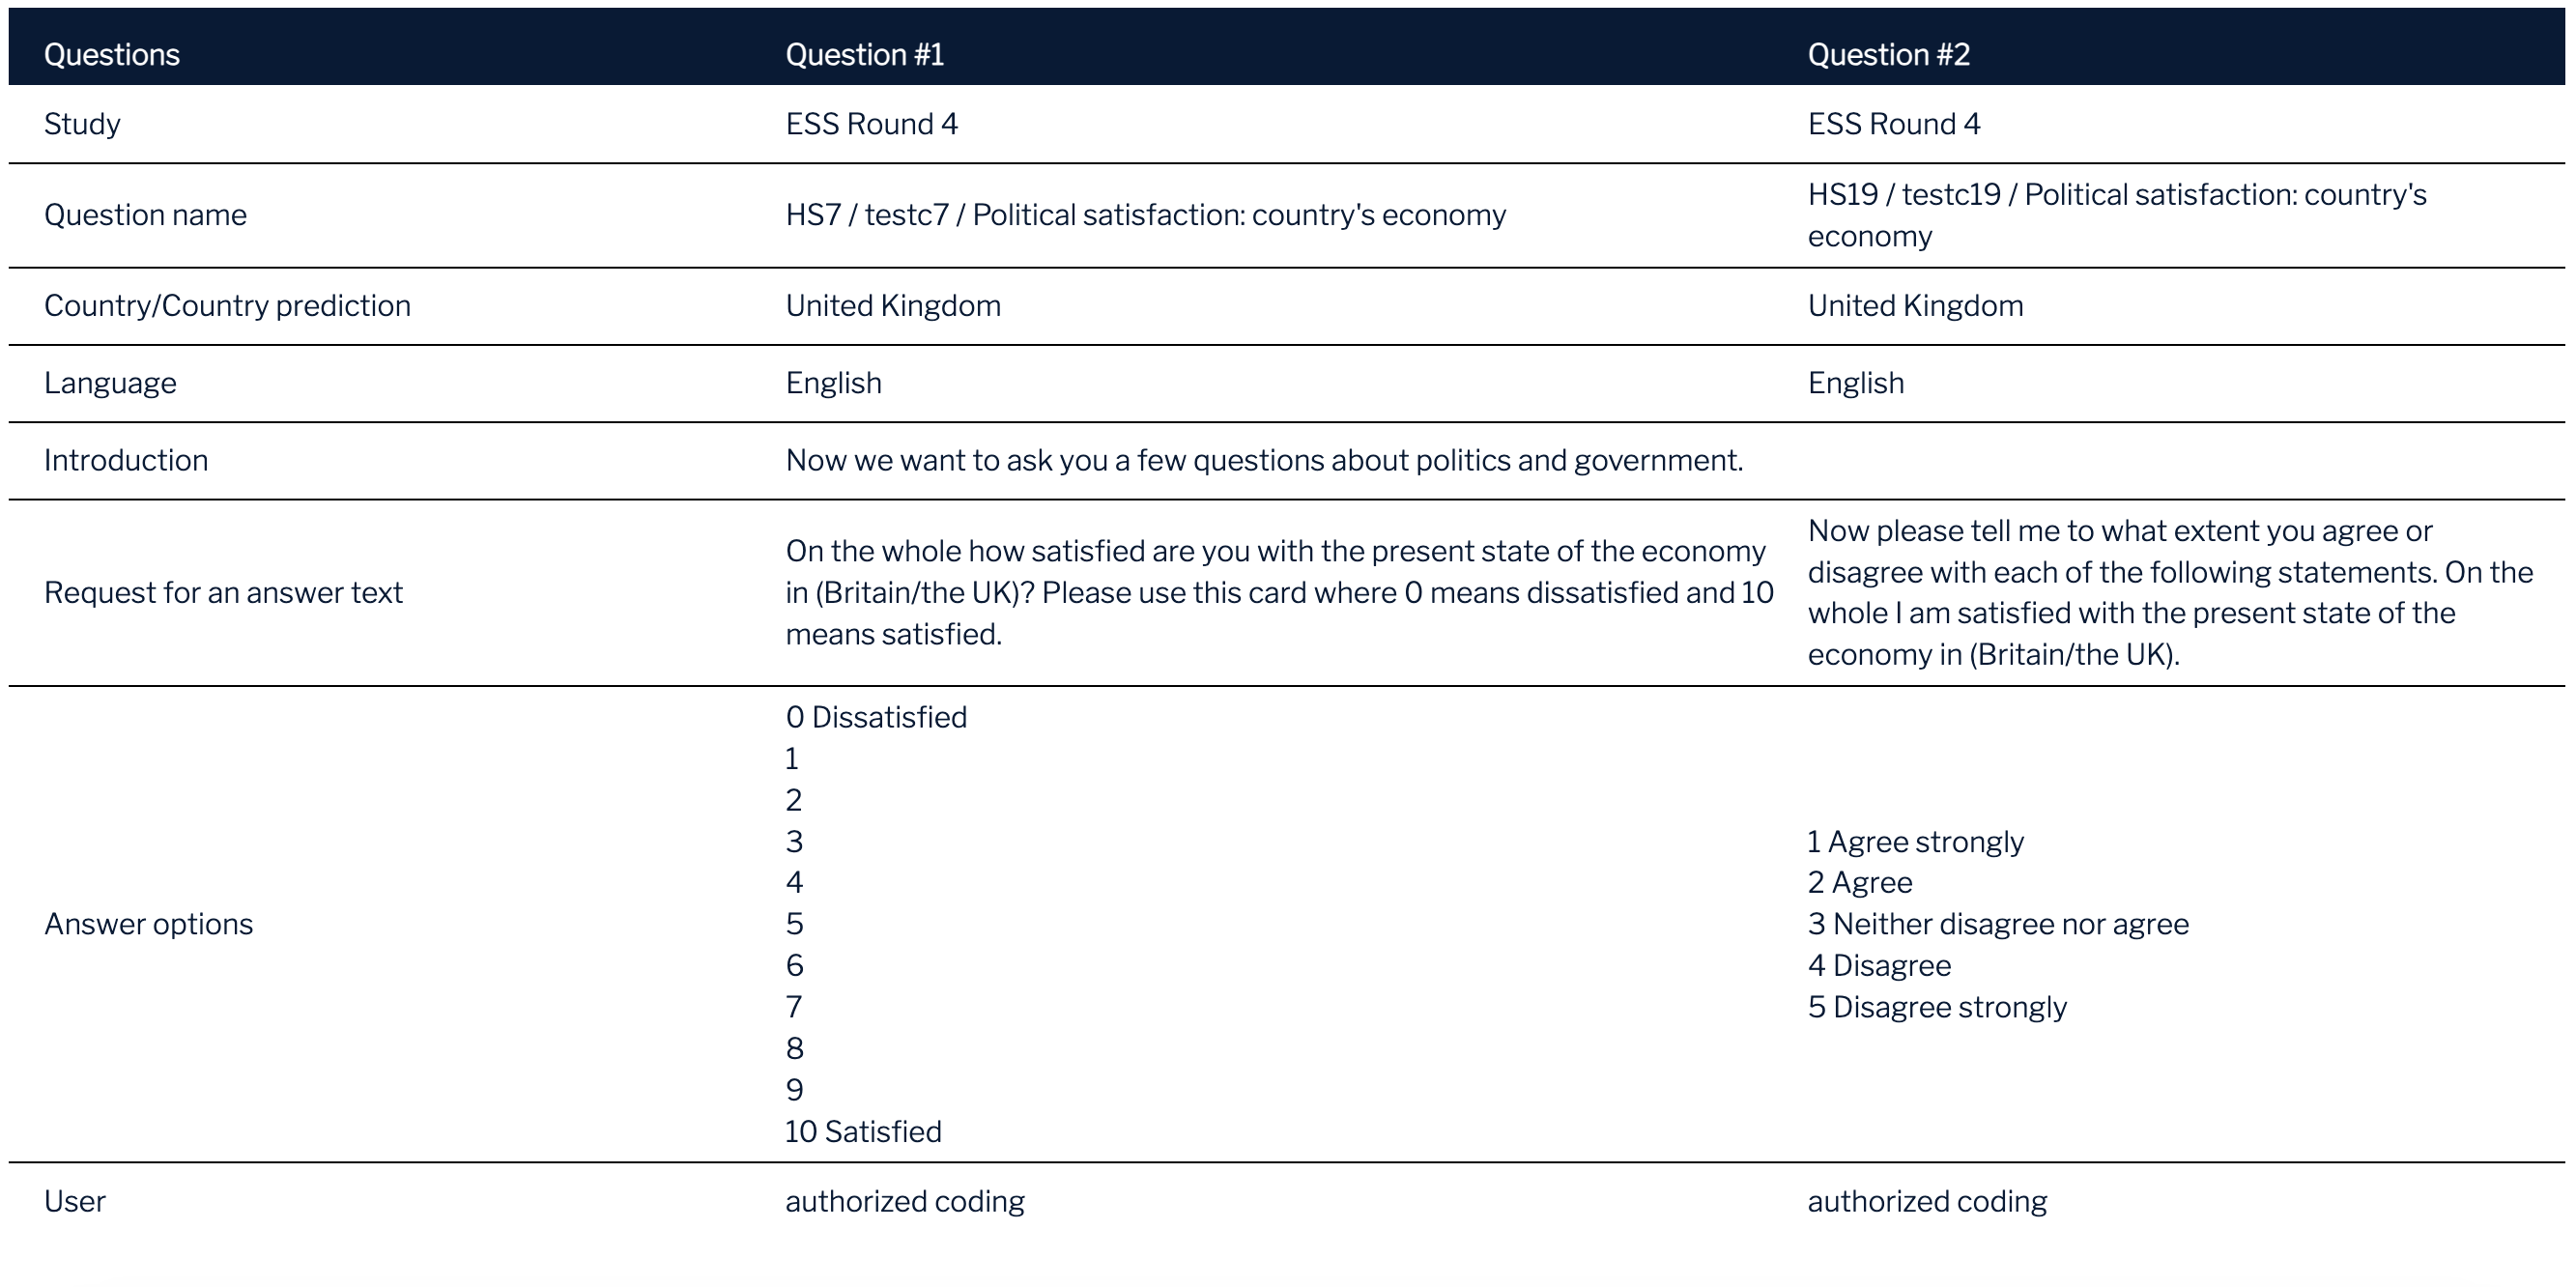
\includegraphics{img/ukeconomy.png}

\begin{itemize}
\item
  The first version ``HS7 / testc7 / Political satisfaction: country's
  economy'' measures the construct using a numeric rating scale that
  ranges from ``0 - Dissatisfied'' to ``10 - Satisfied.'' The question
  asks, ``On the whole, how satisfied are you with the present state of
  the economy in (Britain/the UK)?'' This scale captures various degrees
  of satisfaction along a continuum, providing respondents with a range
  of options to express their attitudes.
\item
  The second version ``HS19 / testc19 / Political satisfaction:
  country's economy'' measures the same construct using a 5-point Likert
  scale with fully labeled response options. The question states, ``To
  what extent do you agree or disagree with the following statement: On
  the whole, I am satisfied with the present state of the economy in
  (Britain/the UK).'' Here, response options range from ``1 - Agree
  strongly'' to ``5 - Disagree strongly,'' categorizing responses into
  distinct levels of agreement or disagreement.
\end{itemize}

\includegraphics{img/domain.png} Using SQP, both survey items were coded
to capture their design characteristics, revealing notable differences.
Shared attributes included the domain, classified as ``National
Politics,'' and the concept of ``Feeling,'' specifically focusing on
satisfaction with the economy. However, variations emerged in other
areas. The numeric scale question was coded as using a symmetric,
theoretically bipolar scale with partially labeled categories,
emphasizing both extremes and intermediate values. In contrast, the
Likert scale question was coded as having fully labeled categories, a
balanced structure, and an indirect request format. Additional
differences included the presence of encouragement to respond in the
Likert scale version, which was absent in the numeric scale question.
These distinctions, highlighted in the coding interface, reflect design
nuances that can influence respondents' interpretations and responses.

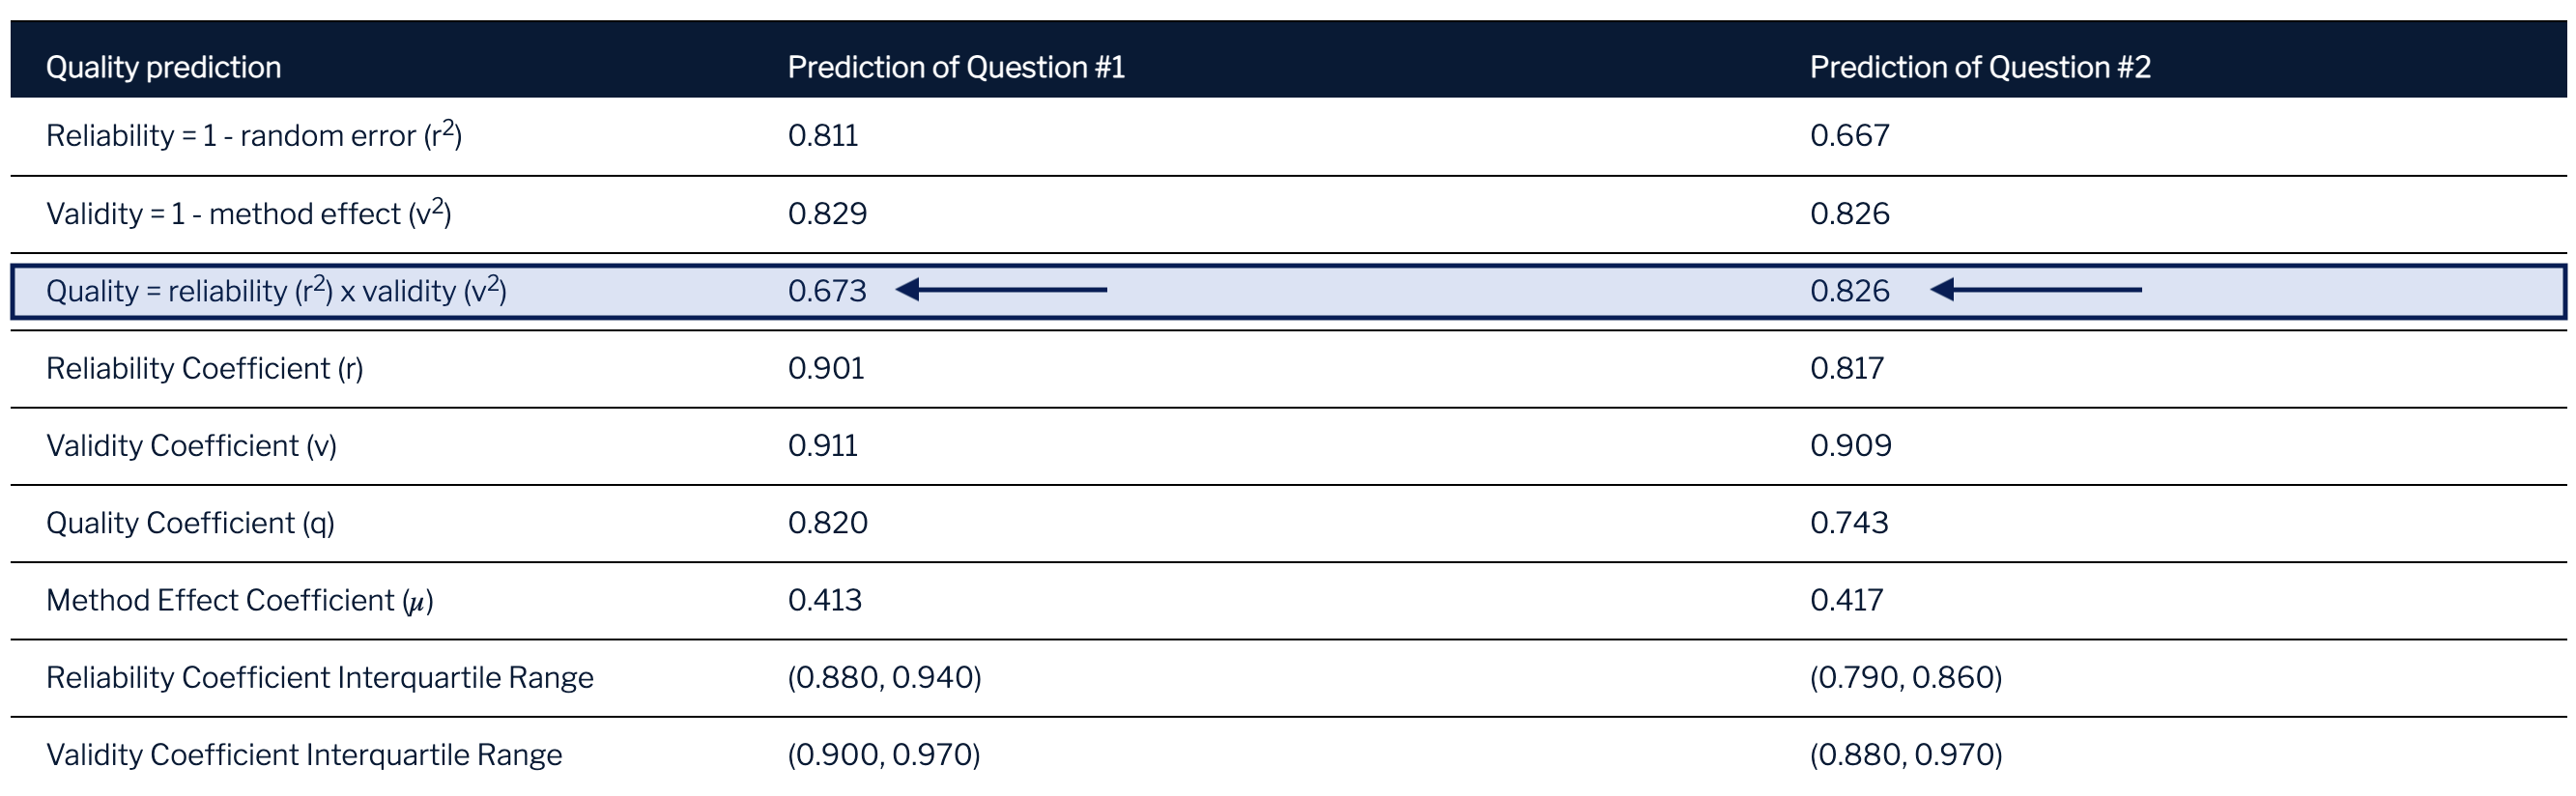
\includegraphics{img/rating.png} SQP generated quality predictions for
both types of questions, highlighting the impact of various design
choices. The numeric rating scale question achieved a reliability score
of \emph{0.811} and a validity score of \emph{0.829}, resulting in an
overall quality score of \emph{0.673}. In contrast, the 5-point Likert
scale question received a reliability score of \emph{0.667} and a
validity score of \emph{0.826}, yielding an overall quality score of
\emph{0.826}. These results emphasize that the Likert scale question,
despite its lower reliability, benefits from higher validity, which
contributes to its superior overall quality score. The findings
illustrate the importance of aligning question design with research
objectives to optimize data quality.

\begin{tcolorbox}[enhanced jigsaw, titlerule=0mm, breakable, toptitle=1mm, leftrule=.75mm, colbacktitle=quarto-callout-note-color!10!white, colback=white, left=2mm, opacitybacktitle=0.6, rightrule=.15mm, opacityback=0, colframe=quarto-callout-note-color-frame, bottomrule=.15mm, arc=.35mm, bottomtitle=1mm, title=\textcolor{quarto-callout-note-color}{\faInfo}\hspace{0.5em}{A Step-by-Step Guide to Hands-on Application}, toprule=.15mm, coltitle=black]

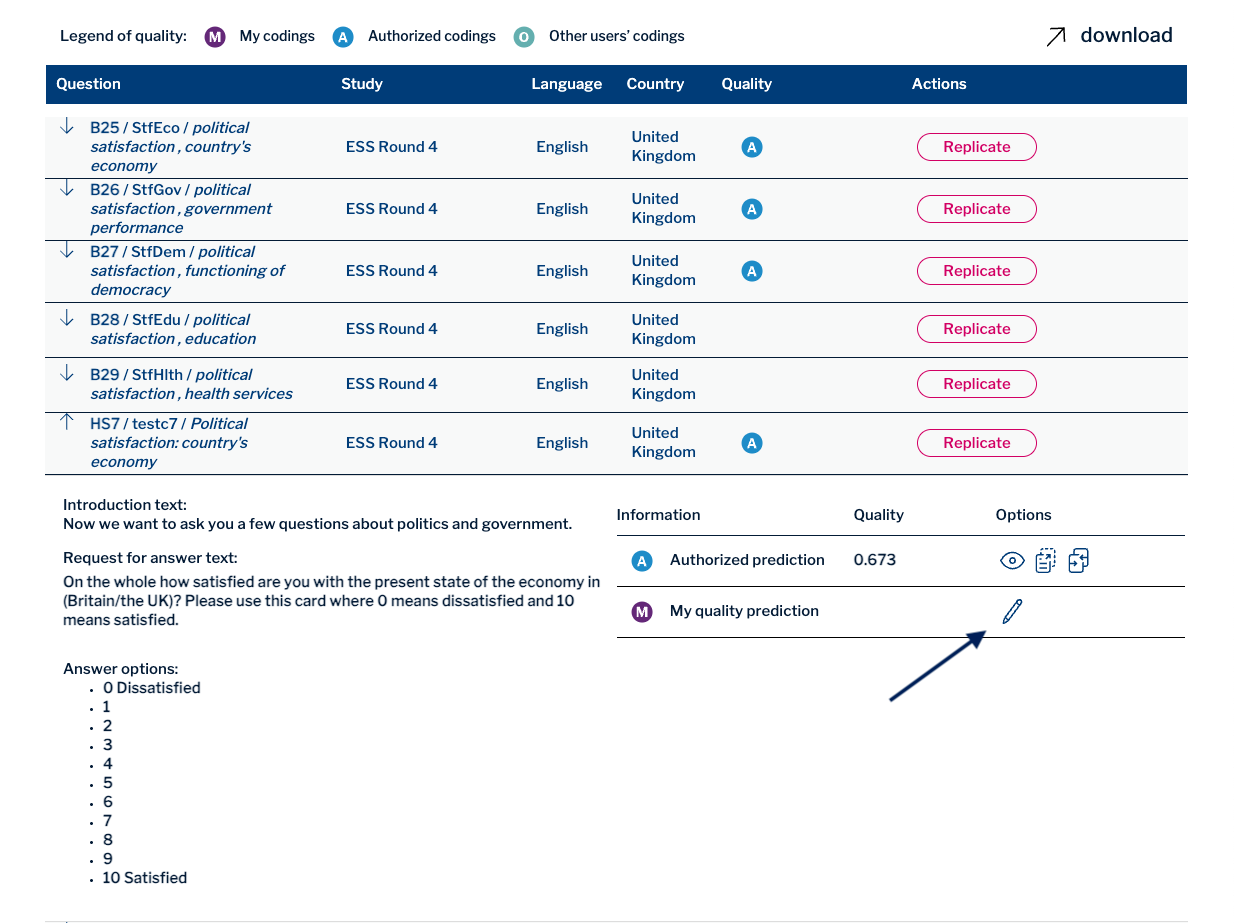
\includegraphics{img/pen.png} \textbf{Step 1:} To begin creating your
own quality prediction, locate the question in the survey item list.
Simply click the pen icon next to the relevant question to open the
coding interface. This will allow you to code the question's
characteristics and predict its measurement quality.

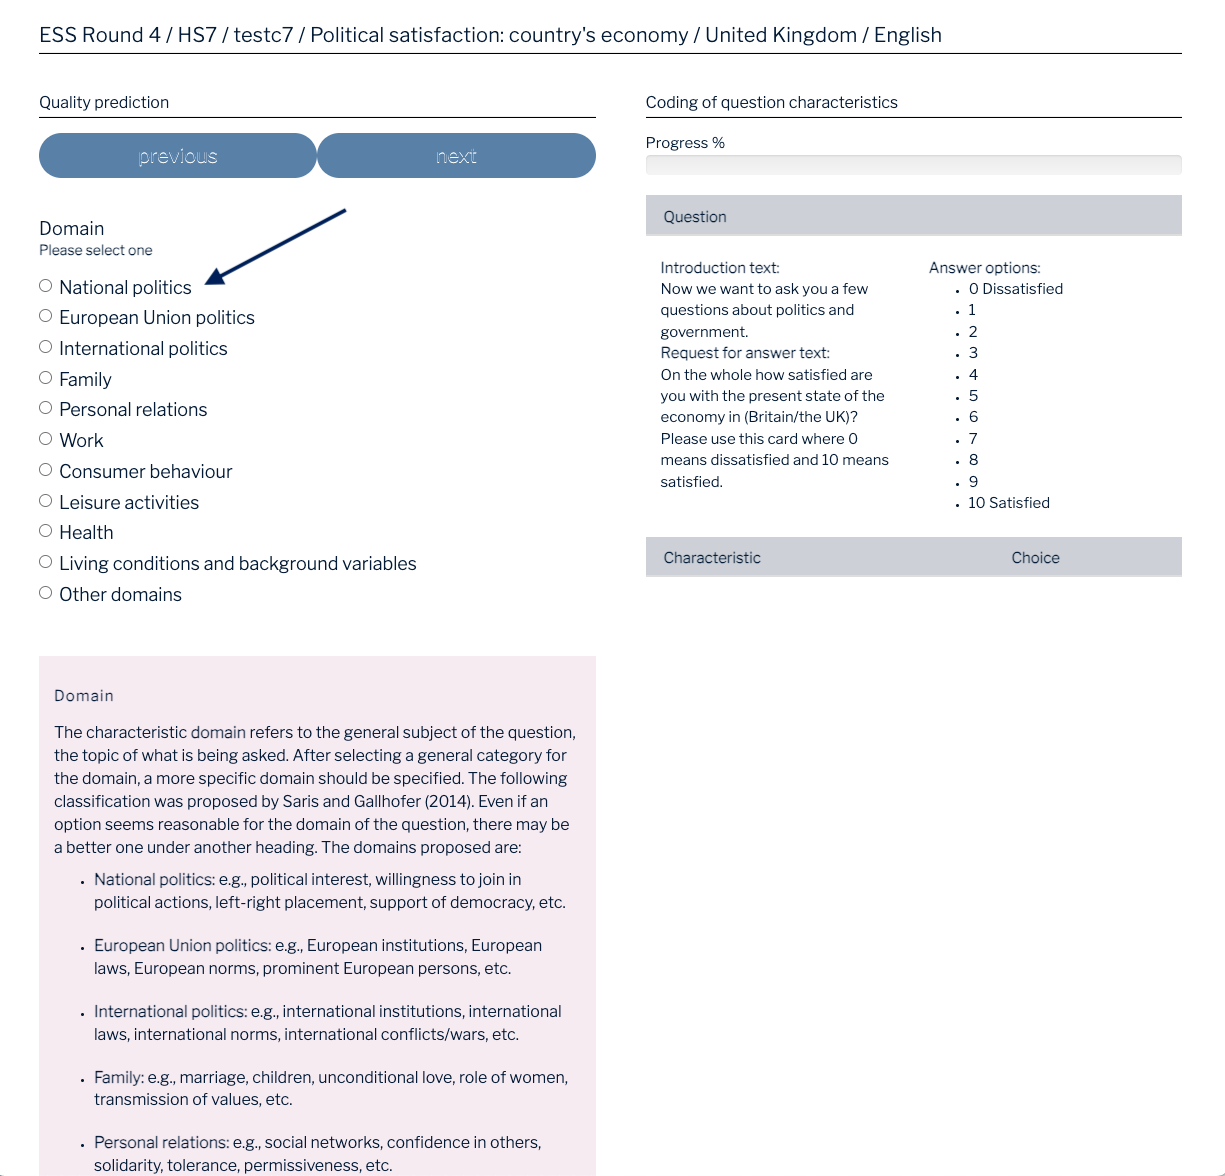
\includegraphics{img/coding.png} \textbf{Step 2:} Once you've accessed
the coding interface, you will start by selecting the appropriate
characteristics for the question. For example, since the question about
satisfaction with the economy pertains to national politics, select
``National politics'' from the list of options. A helpful pink box
appears below the coding options, providing detailed explanations for
each characteristic. Use this guidance to ensure you understand the
options and make accurate selections. After completing this step, click
``Next'' to proceed to the next characteristic.

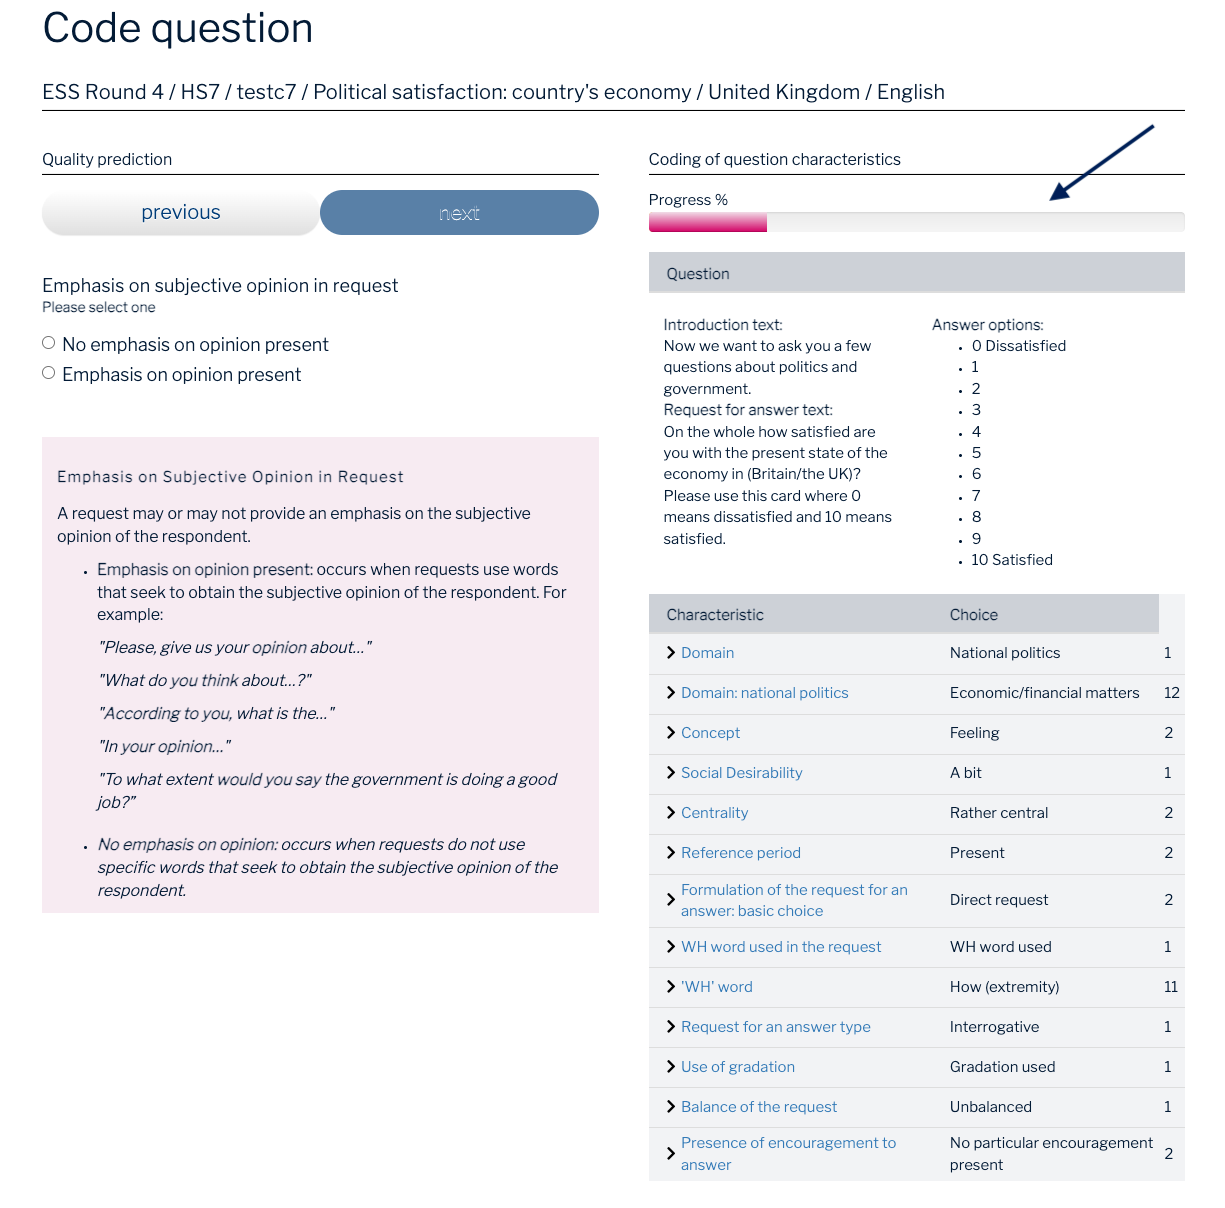
\includegraphics{img/progress.png} \textbf{Step 3:} Repeat the process
for each characteristic of the survey item. As you progress, the
progress bar at the top of the screen will indicate how much of the
coding is complete. On the right-hand side, your previous answers are
displayed, enabling you to review and make corrections if necessary. If
you realize an error or need to adjust a response, simply go back to the
corresponding step and update your selection. Continue coding until the
progress bar is fully completed, ensuring that all characteristics have
been coded accurately.

\textbf{Step 4:} By following these steps, you can generate a reliable
quality prediction for the survey item, gaining valuable insights into
its measurement properties.

\end{tcolorbox}

\section{Conclusion}\label{conclusion}

The Survey Quality Predictor (SQP) is a powerful tool for improving
survey research by enabling a systematic evaluation of question design.
It can predict the reliability, validity, and quality of survey items
based on their formal and linguistic characteristics. This capability is
invaluable for researchers looking to enhance their measurement
instruments. By linking these characteristics to measurement quality,
SQP provides actionable insights for creating better questionnaires,
supports quality control in survey research, and helps reduce potential
biases when measuring subjective concepts such as attitudes and
opinions.

Despite its advantages, SQP has some limitations. Its dependence on user
coding can introduce subjectivity in interpreting the characteristics of
survey questions. While the platform provides authorized codings for
numerous survey questions and offers detailed guidance to minimize this
risk, the quality of predictions can still vary depending on the user's
expertise. Additionally, the coding process---which requires assessing
up to 60 characteristics for each item---can be time-consuming for those
unfamiliar with the tool. Furthermore, although SQP's database is
extensive, it is not exhaustive, and the quality of predictions may not
fully capture the nuances of all survey contexts or emerging
methodologies.

Looking ahead, the potential for SQP's development is promising.
Expanding the database to include more languages, regions, and survey
design choices would enhance its applicability, particularly in
underrepresented contexts. Incorporating large language models to
automate parts of the coding process could alleviate the cognitive load
on users and improve consistency. Additionally, integrating SQP with
newer survey methodologies and adaptive designs, along with continuously
updating its algorithm to reflect advancements in survey research, will
help maintain its relevance in a rapidly evolving field. By addressing
these challenges and embracing innovation, SQP can continue to be an
indispensable tool for survey researchers around the world.

\phantomsection\label{refs}
\begin{CSLReferences}{1}{0}
\bibitem[\citeproctext]{ref-andrews1984}
Andrews, F. M. (1984). Construct validity and error components of survey
measures: {A} structural modeling approach. \emph{Public Opinion
Quarterly}, \emph{48}(2), 409--442. \url{https://doi.org/10.1086/268840}

\bibitem[\citeproctext]{ref-felderer2024}
Felderer, B., Repke, L., Weber, W., Schweisthal, J., \& Bothmann, L.
(2024). \emph{Predicting the {Validity} and {Reliability} of {Survey}
{Questions}}. Open Science Framework.
\url{https://doi.org/10.31219/osf.io/hkngd}

\bibitem[\citeproctext]{ref-gesis2024}
GESIS -- Leibniz Institute for the Social Sciences. (2024). \emph{User
{Manual} for {SQP} 3.0}. GESIS -- Leibniz Institute for the Social
Sciences. \url{https://sqp.gesis.org}

\bibitem[\citeproctext]{ref-saris2014}
Saris, W. E., \& Gallhofer, I. N. (2014). \emph{Design, {Evaluation},
and {Analysis} of {Questionnaires} for {Survey} {Research}} (2nd
Edition). Wiley.

\bibitem[\citeproctext]{ref-saris2022}
Saris, W. E., Oberski, D., \& Weber, W. (2022). \emph{The {Quality} of
{Survey} {Questions} for {Continuous} {Latent} {Variables}: {Your}
{Guide} to the {SQP} {Database} \& {Predictions}}. Independently
Published.

\bibitem[\citeproctext]{ref-saris2016}
Saris, W. E., \& Revilla, M. (2016). {Correction for Measurement Errors
in Survey Research: Necessary and Possible}. \emph{Social Indicators
Research: An International and Interdisciplinary Journal for
Quality-of-Life Measurement}, \emph{127}(3), 1005--1020.
\url{https://doi.org/10.1007/s11205-015-1002-x}

\end{CSLReferences}




\end{document}
